% Svolgimento B63-E01 (prova del 15/03/2021): cilindro in corrente a M = 10, schlieren.
% Numeri e figure: calcoli.py (stessa cartella). Compilare con: latexmk -pdf svolgimento.tex

\documentclass[11pt,a4paper]{article}

% --- Preambolo di fonti/formulario.tex ---
\usepackage[T1]{fontenc}
\usepackage[utf8]{inputenc}
\usepackage[italian]{babel}
\usepackage{amsmath,amssymb}
\usepackage[a4paper,margin=2.5cm]{geometry}
\usepackage{array}

% --- Pacchetti aggiuntivi per gli svolgimenti ---
\usepackage{siunitx}
\usepackage{booktabs}
\usepackage{graphicx}
\usepackage{float}
\usepackage{hyperref}

\hypersetup{hidelinks}
\setlength{\parindent}{0pt}
\setlength{\parskip}{4pt}
\allowdisplaybreaks
\graphicspath{{figure/}}

\sisetup{output-decimal-marker={,}, group-separator={\,}, per-mode=symbol,
         exponent-product=\cdot, range-phrase={\text{--}}}

\newcommand{\Vv}{\boldsymbol V}
\newcommand{\Cp}{C^{+}}
\newcommand{\Cm}{C^{-}}
\newcommand{\F}[1]{(F~\S#1)}
\newcommand{\Sm}[1]{(S~p.~#1)}

\title{Gasdinamica -- Svolgimento \texttt{B63-E01}\\[2pt]
\large Cilindro in corrente supersonica a $M_\infty=10$: lettura della schlieren}
\author{}
\date{Prova del 15/03/2021}

\begin{document}
\maketitle

\section*{Traccia}
\emph{Nella figura vediamo un'immagine schlieren di un flusso supersonico, stazionario, piano, a numero
di Mach pari a 10, che investe un cilindro. Analizzare il campo di moto e descrivere le sue
caratteristiche principali. Determinare: a) la stand-off distance dell'urto; b) la posizione della
linea sonica nel punto di intersezione di questa con il cilindro; c) il numero di Mach nel punto di
separazione; d) la pressione media nella bolla di ricircolo; e) il numero di Mach a monte dell'urto
nella zona di riattacco della scia. Riportare le stime fatte sul piano odografo e su quello
$p$--$\theta$.} (Nella traccia l'ultima domanda è etichettata di nuovo ``d)''; qui la chiamo e).)

La traccia coincide con B63-E01 del catalogo. L'ho risolta in modo indipendente: misure e
modelli sono descritti qui sotto.

%==============================================================================
\section{Lettura del testo e dell'immagine}

\begin{figure}[H]
  \centering
  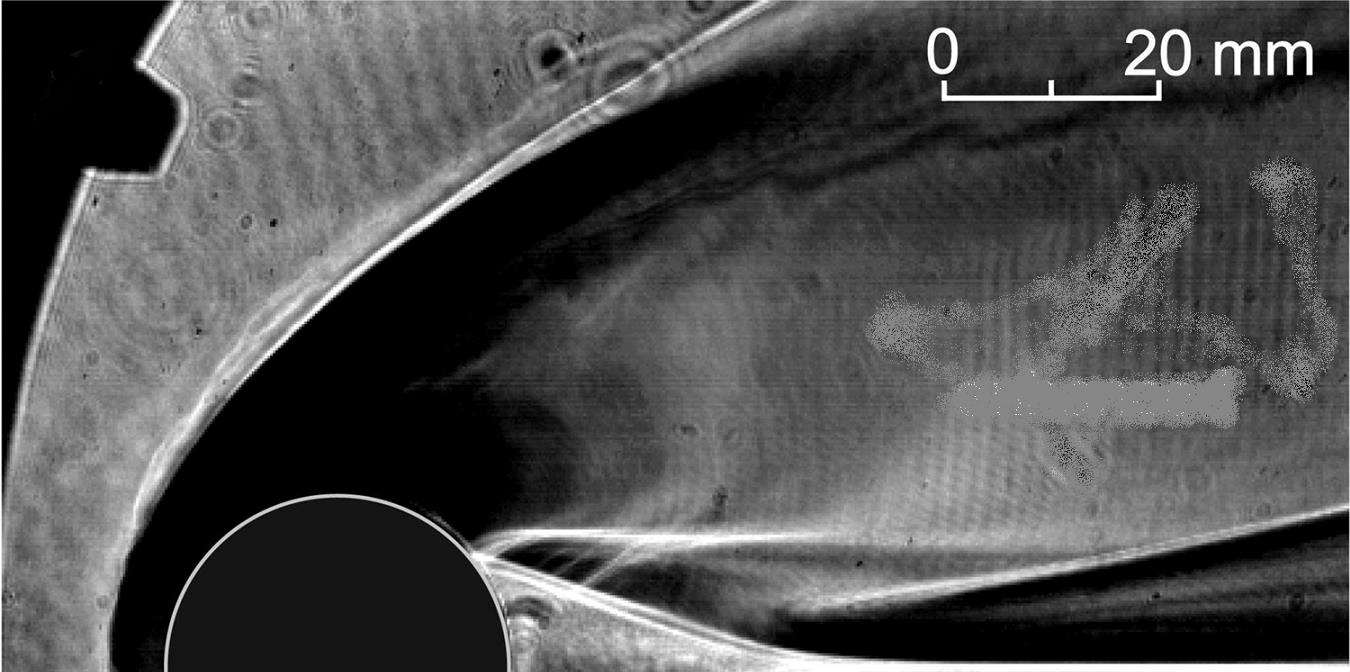
\includegraphics[width=0.85\textwidth]{originale_scansione.jpg}
  \caption{Schlieren della traccia (immagine estratta dalla scansione del testo d'esame, più
  nitida della fotografia dello schermo, salvata come \texttt{figure/originale.jpg}). Corrente da
  sinistra verso destra; il bordo inferiore coincide, a meno di pochi pixel, con l'asse di simmetria.}
  \label{fig:orig}
\end{figure}

\paragraph{Cosa mostra.} La metà superiore del campo attorno a un cilindro (il disco nero, con il
contorno evidenziato da un anello chiaro aggiunto all'immagine), investito da una corrente
uniforme a $M_\infty=10$ che va da sinistra a destra. Il bordo inferiore dell'immagine passa per il centro del cilindro:
quindi è l'asse di simmetria (il campo è simmetrico per ipotesi: corrente piana, cilindro, incidenza nulla).

\paragraph{Tecnica.} Una schlieren rende visibili i \emph{gradienti} di densità (in una direzione,
quella del coltello): le discontinuità sottili (urti) appaiono come linee nette chiare o scure, gli
strati di scorrimento come bande più sfumate, le regioni a densità uniforme come zone a
luminosità uniforme. Il valore assoluto della luminosità non dà la densità: posso usare
l'immagine solo per \emph{posizioni e inclinazioni} delle strutture.

\paragraph{Regime.} La traccia dice che la corrente è stazionaria. Nell'immagine l'urto di prua e
gli urti della scia sono nitidi, cosa compatibile con la stazionarietà (un'immagine di un campo
instazionario a lunga esposizione li sfumerebbe). Fa eccezione la scia vicina, che ha una
tessitura irregolare: è il ricircolo, di natura instazionaria e turbolenta.

\paragraph{Scala e riferimenti.} La barra 0--\SI{20}{mm} (tacche a 0, 10, \SI{20}{mm}) dà
$\num{10.72}$ px/mm. L'asse di simmetria è orizzontale e coincide con la direzione della corrente
indisturbata: è il riferimento per gli angoli ($\theta$ positivo antiorario, \F{10}). Le
macchie grigie a destra (lettere ritoccate) sono artefatti di stampa. Lo stesso vale per la cornice
dentellata a sinistra, che è il bordo della finestra ottica.

\paragraph{Dati e richieste.}
\begin{table}[H]
  \centering
  \begin{tabular}{lll}
    \toprule
    Grandezza & Valore & Note \\
    \midrule
    $M_\infty$ & \num{10} & dato \\
    $\gamma$ & \num{1.4} & aria (assunto: la traccia non lo specifica) \\
    $p_1$ & \num{1} & pressione di riferimento: i risultati sono rapporti $p/p_1$ \\
    scala & \SI{20}{mm} $\leftrightarrow$ \num{214.5} px & barra sull'immagine \\
    \bottomrule
  \end{tabular}
  \caption{Dati. Le grandezze geometriche (raggio, angoli) vanno misurate sull'immagine.}
\end{table}
Le richieste sono cinque stime, a)--e), e le rappresentazioni sui piani odografo e $p$--$\theta$. Tutte, tranne
il Mach indisturbato, dipendono da misure sull'immagine: sono \emph{stime}, e per ognuna riporto
l'incertezza.

%==============================================================================
\section{Identificazione delle strutture}
Le elenco nell'ordine in cui le incontra una particella che viaggia da sinistra verso destra (fig.~\ref{fig:ann}).

\begin{enumerate}
\item \textbf{Urto di prua (bow shock), staccato.} È la linea netta curva davanti al cilindro.
  Il cilindro è un corpo tozzo: la deviazione imposta dalla parete supera $\theta_{\max}(10)=\ang{44.4}$, quindi
  un urto attaccato è impossibile. Inoltre un urto da solo non può portare la velocità a zero
  ($u_2/u_1\ge(\gamma-1)/(\gamma+1)$). L'urto si stacca dunque a distanza finita (stand-off) e la
  corrente rallenta, in modo subsonico, fino al punto di ristagno. Sull'asse l'urto è normale,
  poi si inclina progressivamente. Lontano dal corpo dovrebbe tendere alla linea di Mach
  $\mu_\infty=\ang{5.74}$: nella parte alta dell'immagine è ancora inclinato di circa \ang{33}, e
  quindi è ancora un urto forte. L'urto resta sottile perché le caratteristiche vi convergono.
\item \textbf{Regione subsonica al naso} (zona scura fra l'urto e il cilindro), chiusa dalla
  \textbf{linea sonica}. La linea sonica va dall'urto al corpo e non si vede nella schlieren:
  la sua intersezione con il cilindro va stimata (domanda b).
\item \textbf{Espansione lungo la parete.} Oltre la linea sonica la corrente diventa supersonica
  e si espande attorno alla parete convessa: è un ventaglio $\Cp$ che nasce dalla parete (che sta sotto la
  corrente). È la regione scura fra urto e corpo, a destra della linea sonica.
\item \textbf{Strato d'entropia.} Le linee di corrente vicine al corpo hanno attraversato la parte
  quasi normale dell'urto, cioè la più intensa: hanno entropia massima e pressione totale $p_0'$
  minima. L'urto è curvo, quindi l'entropia varia da una linea di corrente all'altra e il
  campo a valle è rotazionale (Crocco, \F{18}).
\item \textbf{Separazione} (punto S, a circa \ang{38} dal punto di ristagno posteriore). È il punto in cui
  la corrente si stacca dalla parete. La causa è viscosa: lo strato limite non sopporta la
  ricompressione verso la base. Un modello non viscoso non sa prevedere la posizione di S,
  che quindi prendo dall'immagine.
\item \textbf{Urto di separazione} (lip shock), la linea chiara quasi orizzontale che parte
  dalla zona di S. Alla separazione la corrente, che scendeva tangente alla parete (circa
  $-\ang{52}$), viene raddrizzata nella direzione dello strato di scorrimento (circa $-\ang{18}$): è
  una \emph{compressione}, onda $\Cp$. Le onde di compressione nascono dallo strato che si incurva e
  coalescono in un urto un po' lontano dalla parete. Ne segue che la linea di corrente adiacente allo strato è
  compressa in modo (quasi) isentropico, mentre quelle più esterne attraversano l'urto. Lo verifico al §\ref{sec:ver}.
\item \textbf{Strato di scorrimento} (shear layer). È la banda chiara che parte da S e scende verso l'asse
  con un'inclinazione di circa \ang{18}. Separa la corrente esterna supersonica dalla bolla. È più
  sfumato degli urti e si allarga verso valle, come ci si aspetta da una discontinuità
  linearmente degenere, resa per di più viscosa e turbolenta dal mescolamento.
\item \textbf{Bolla di ricircolo} (B), la regione a tessitura irregolare fra lo strato, la base del
  cilindro e l'asse. Il fluido vi ricircola a bassa velocità: in prima approssimazione la
  pressione è uniforme e uguale a quella della corrente che la lambisce.
\item \textbf{Collo della scia} (neck), dove lo strato raggiunge l'asse, a circa
  \SI{43}{mm} dal centro del cilindro. Qui le due correnti simmetriche si incontrano e devono tornare parallele all'asse.
\item \textbf{Urto di ricompressione o di riattacco} (C$^+$, linea netta che sale dalla zona del
  collo). Riallinea la corrente all'asse ($-\ang{18}\to\ang{0}$). Ha il piede nello strato a monte del
  collo e si incurva verso l'alto, perché si forma per coalescenza delle compressioni con cui lo strato si
  raddrizza. Più a valle (circa $x=\SI{116}{mm}$ dal bordo) incrocia l'urto di separazione.
\item \textbf{Scia a valle} (regione 6): corrente di nuovo parallela all'asse, con al centro la scia
  viscosa.
\end{enumerate}
\textbf{Artefatti:} l'anello chiaro attorno al cilindro (disegnato), la cornice dentellata a
sinistra (finestra), le lettere ritoccate a destra, le frange regolari (difetti
dell'ottica).

%==============================================================================
\section{Ipotesi ancorate all'immagine}
\begin{itemize}
\item \emph{Stazionario, piano, simmetrico} (dato; l'immagine è coerente: urti nitidi, asse orizzontale per il
  centro del cilindro). Studio solo la metà superiore. Al posto della parete inferiore c'è l'asse di simmetria,
  che si comporta come una parete ($\theta=0$).
\item \emph{Gas perfetto, $\gamma=1{,}4$, non viscoso fuori dagli strati sottili}. La viscosità
  conta solo nello strato limite, nello strato di scorrimento e nella bolla, ma è la
  causa della separazione: per questo la posizione di S \emph{si misura e non si calcola}.
\item \emph{Entalpia totale uniforme}: stazionario e adiabatico, $h_0$ si conserva anche attraverso gli
  urti. Quindi $a^*$ è unico in tutto il campo e c'è un solo piano odografo per tutti gli stati \F{13}.
\item \emph{La corrente che lambisce il corpo ha la pressione totale di ristagno $p_0'$}: la linea di corrente di
  parete viene dal punto di ristagno, quindi ha attraversato l'urto \emph{normale}. Lungo di essa il moto è
  isentropico, perché non attraversa altri urti fino a W (questo va verificato).
\item \emph{Espansione lungo la parete come onda semplice $\Cp$} (fra la linea sonica e S): trascuro le onde
  riflesse dall'urto di prua e dalla linea sonica. È un'ipotesi approssimata, e la discuto al §\ref{sec:disc}.
\item \emph{Corrente W uniforme} fra la separazione e il piede dell'urto di riattacco, diretta come lo strato di
  scorrimento ($\theta_W=-\Delta\theta$). La bolla è a pressione uniforme $p_B=p_W$: un ricircolo lento non
  sostiene gradienti di pressione apprezzabili.
\item \emph{Contorno dello strato come parete}: lo strato di scorrimento impone la direzione alla corrente esterna. Lo
  dice la condizione di raccordo su una linea di scorrimento \F{13}: stessa $p$, stessa $\theta$.
\end{itemize}
In sintesi, \textbf{l'immagine dà} le posizioni e le inclinazioni (stand-off, raggio, $\theta_s$,
$\Delta\theta$, inclinazione dell'urto di riattacco). \textbf{Si assumono} $\gamma$, l'assenza di onde
riflesse lungo la parete, l'uniformità di W e della pressione nella bolla.

%==============================================================================
\section{Misure sull'immagine}\label{sec:mis}
Ho fatto le misure in coordinate pixel sull'immagine della fig.~\ref{fig:orig} ($1350\times672$ px), con
$x$ verso destra e $y$ verso il basso. Ho individuato le linee come creste di luminosità (o fronti
chiaro/scuro) colonna per colonna e le ho interpolate ai minimi quadrati. Equivale a
tracciare le linee e misurarle con righello e goniometro, ma con un'incertezza controllabile.

\begin{table}[H]
  \centering
  \small
  \begin{tabular}{p{3.3cm}p{5.4cm}p{5.6cm}}
    \toprule
    Misura & Valore & Come / incertezza \\
    \midrule
    Scala & $\num{214.5}$ px $=\SI{20}{mm}$ $\Rightarrow$ \num{10.72} px/mm & tacche della barra; $\pm1$ px ($\pm\SI{0.5}{\%}$) \\
    Cilindro & centro $(337{,}0;\,666{,}6)$ px, $R=\num{171.2}$ px $=\SI{15.96}{mm}$ ($D\simeq\SI{32}{mm}$) & fit di una circonferenza su 300 punti dell'anello; $\pm1{,}5$ px \\
    Asse di simmetria & $y=\num{666.6}$ px & orizzontale per il centro \\
    Urto sull'asse & $x=105$ px; naso $x=165{,}8$ px & cresta dell'urto nelle righe vicine all'asse; $\pm4$ px (spessore della cresta) \\
    \textbf{Stand-off} & $\Delta=60{,}8$ px $=\SI{5.7(4)}{mm}$, $\Delta/R=\num{0.355(30)}$ & \\
    Separazione S & $\theta_s=\ang{38}\pm\ang{3}$ dal ristagno posteriore & intersezione dello strato (primo tratto) con il cerchio \\
    Strato di scorrimento & \ang{19.0} (primo tratto), \ang{16.5} (prima del collo) & adotto $\Delta\theta=\ang{18}\pm\ang{1.5}$ \\
    Urto di riattacco (inclinazione sull'asse) & piede \ang{7.8}; tratto formato \ang{12.1}; oltre l'incrocio \ang{14.0} & adotto il tratto formato: $\sigma_{ax}=\ang{12}\pm\ang{1}$ \\
    Urto di separazione & $+\ang{0.2}\pm\ang{0.2}$ (orizzontale) & tratto $x=500$--$880$ px \\
    Urto di prua, parte alta & circa \ang{33} sull'orizzontale ($y\simeq\SI{45}{mm}$ dall'asse) & solo qualitativa \\
    \bottomrule
  \end{tabular}
  \caption{Misure sull'immagine (calcoli.py, parte 1).}
\end{table}

\paragraph{Quale inclinazione per l'urto di riattacco.} L'urto è curvo: la sua inclinazione sale
da circa \ang{8} al piede a circa \ang{12} nel tratto prima dell'incrocio con l'urto di separazione
($x\simeq\num{1250}$ px), e oltre l'incrocio arriva a \ang{14}. Il motivo è che l'urto nasce per
\emph{coalescenza} delle onde di compressione con cui lo strato si raddrizza verso l'asse.
Succede la stessa cosa con la compressione su una parete concava (o con il pistone in $x$--$t$): al piede
l'urto raccoglie solo una parte della deviazione ed è più debole e meno inclinato. Solo dopo la
coalescenza porta tutta la deviazione $\Delta\theta$. Oltre l'incrocio, invece, lo stato a monte non è più W. La relazione
$\theta$--$\sigma$--$M$ con $\theta=\Delta\theta$ vale quindi nel tratto formato: adotto
$\sigma_{ax}=\ang{12}\pm\ang{1}$. Al §\ref{sec:disc} mostro che il valore del piede dà risultati incoerenti.

%==============================================================================
\section{Ricostruzione del campo}

\subsection{Modello e ipotesi}
\begin{itemize}
\item \textbf{Naso (regione subsonica):} lungo la linea di ristagno uso solo relazioni esatte. Sono
  l'urto normale \F{5} e la decelerazione isentropica fino al ristagno, che dà $p_0'$. Il modello 2D supersonico
  non vale qui (regione subsonica, ellittica), e infatti non lo uso.
\item \textbf{Parete, separazione, scia:} 2D stazionario supersonico \F{10--13}, cioè onde di
  Prandtl--Meyer \F{11} e urti obliqui \F{12}. Vale perché tutte le regioni coinvolte (dalla linea
  sonica in poi: S, W, 6) risultano supersoniche: lo verifico a posteriori.
\item \textbf{Stand-off:} la teoria del corso non dà una formula chiusa. Il valore richiesto è quello
  \emph{misurato}. Lo confronto con la correlazione empirica di Billig (fuori formulario).
\item \textbf{Linea sonica sul corpo:} due stime indipendenti. (i) La catena di onde dalla scia alla
  parete (invariante $\theta+\nu$). (ii) La regola di Busemann del corso \F{18}: il punto sonico
  sul corpo è dove la pendenza della parete uguaglia la deviazione sonica della polare di
  $M_\infty$ (rampa equivalente che dà lo stesso salto di Mach).
\end{itemize}

\subsection{Analisi qualitativa}
Seguendo una linea di corrente vicina al corpo:
\begin{enumerate}
\item urto normale (compressione) $1\to2$: $M$ crolla a valori subsonici, l'entropia sale e $p_0$ crolla;
\item compressione isentropica subsonica fino al ristagno ($p=p_0'$), poi riaccelerazione lungo la parete;
  $M=1$ nel punto 3 (linea sonica);
\item espansione supersonica $\Cp$ lungo la parete convessa: $\theta$ diminuisce, $\nu$ cresce, mentre
  $\theta+\nu$ resta costante (onda semplice $\Cp$, \F{11}) fino a S;
\item alla separazione la corrente devia nel verso opposto ($\theta$ cresce da $-\ang{52}$ a
  $-\ang{18}$): compressione $\Cp$. Se è isentropica, \emph{conserva lo stesso invariante}
  $\theta+\nu$ (stessa famiglia), quindi W sta sulla stessa curva di parete;
\item al collo, compressione $\Cp$ da $-\ang{18}$ a \ang{0}, attraverso l'urto di riattacco (urto vero, ben formato): $W\to6$.
\end{enumerate}
Ordini di grandezza attesi: $p_B$ molto minore di $p_0'$ (la base di un corpo tozzo è in depressione, al più
dell'ordine di $p_\infty$), $p_6>p_B$ (ricompressione), e $M$ alla separazione molto alto, perché l'espansione
attorno al cilindro supera i \ang{90}.

\subsection{Topologia del campo}
\begin{table}[H]
  \centering
  \small
  \begin{tabular}{cp{7.2cm}p{6.4cm}}
    \toprule
    Stato & Posizione & Separato dal precedente da \\
    \midrule
    1 & corrente indisturbata ($M=10$, $\theta=0$) & -- \\
    2 & subito a valle dell'urto, sull'asse & urto di prua (normale sull'asse) \\
    0$'$ & punto di ristagno anteriore ($p=p_0'$) & compressione isentropica subsonica \\
    3 & punto sonico sul cilindro ($M=1$, $\theta=\theta^*$) & ricompressione/riaccelerazione subsonica \\
    S & parete subito a monte della separazione ($\theta=-(90^\circ-\theta_s)$) & ventaglio $\Cp$ di espansione lungo la parete \\
    W & corrente esterna lungo lo strato ($\theta=-\Delta\theta$) & compressione $\Cp$ (isentropica) alla separazione \\
    B & bolla di ricircolo ($p_B=p_W$, $V\simeq0$) & strato di scorrimento \\
    6 & a valle dell'urto di riattacco ($\theta=0$) & urto obliquo $\Cp$ di riattacco \\
    \bottomrule
  \end{tabular}
  \caption{Stati e onde (metà superiore; per simmetria la metà inferiore è speculare, con onde $\Cm$).}
\end{table}

\begin{figure}[H]
  \centering
  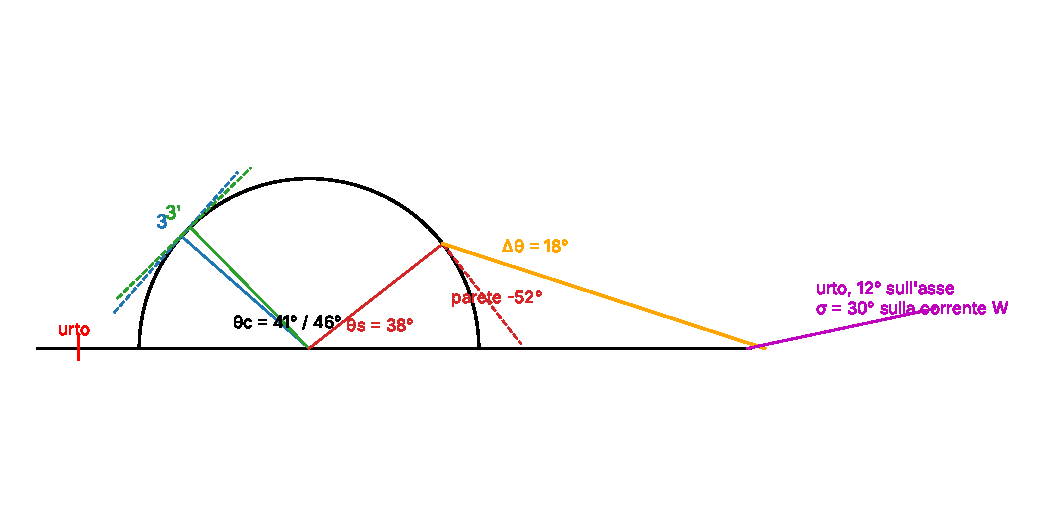
\includegraphics[width=0.9\textwidth]{schema.pdf}
  \caption{Schema geometrico in unità di $R$: semicirconferenza, punto sonico (3 dalla catena, 3$'$
  dalla regola di Busemann) con la tangente, separazione a $\theta_s$ con la direzione della parete,
  strato di scorrimento a $\Delta\theta$ e urto di riattacco.}
  \label{fig:schema}
\end{figure}

\subsection{Bilancio equazioni/incognite}
Le incognite della catena scia--parete sono $M_W$, $M_S$ e $\theta^*$ (cioè la posizione del punto sonico). Le equazioni sono:
\begin{itemize}
\item la relazione $\theta$--$\sigma$--$M$ per l'urto di riattacco, con $\theta=\Delta\theta$ e $\sigma$ misurati: dà $M_W$;
\item l'invariante $\theta+\nu$ della compressione isentropica alla separazione, con $\theta_S$ misurato: dà $M_S$;
\item l'invariante $\theta+\nu$ dell'onda semplice lungo la parete, con $M=1$ ($\nu=0$) al punto sonico: dà $\theta^*$.
\end{itemize}
Sono tre equazioni in tre incognite. La pressione nella bolla segue da $p_0'$ e $M_W$. La regola di
Busemann dà un'equazione \emph{in più} per $\theta^*$: il sistema è sovradeterminato e la differenza fra le due
stime misura la coerenza fra il modello e l'immagine.

\subsection{Scorciatoie fisiche}
\begin{itemize}
\item \textbf{Stessa famiglia, stesso invariante.} Espansione lungo la parete e compressione alla
  separazione sono entrambe onde $\Cp$ isentropiche, quindi
  $\theta+\nu=\text{cost}$ da 3 fino a W: $\theta^*+0=\theta_S+\nu_S=\theta_W+\nu_W$. Ne segue che
  \emph{la posizione del punto sonico dipende solo da W}, non da $\theta_s$ (misura incerta) né da $M_S$ (mal
  condizionato).
\item \textbf{$h_0$ uniforme} $\Rightarrow$ un solo $a^*$ $\Rightarrow$ un solo odografo; per l'urto normale
  vale $M_1^*M_2^*=1$ \F{13}.
\item \textbf{$p_0'$ dalla linea di ristagno}: l'urto normale è esatto sull'asse, quindi la pressione totale di
  tutta la corrente di parete è nota senza conoscere la forma dell'urto.
\end{itemize}

%==============================================================================
\subsection{Calcolo}

\subsubsection*{Stato 1 e urto normale sull'asse (stato 2, ristagno 0$'$)}
Dall'urto normale \F{5} con $M_1=10$, $\gamma=1{,}4$:
\[
\frac{p_2}{p_1}=1+\frac{2\gamma}{\gamma+1}(M_1^2-1)=1+\frac{2{,}8}{2{,}4}\cdot 99=\num{116.5},\qquad
\frac{\rho_2}{\rho_1}=\frac{(\gamma+1)M_1^2}{(\gamma-1)M_1^2+2}=\frac{240}{42}=\num{5.714},
\]
\[
M_2^2=\frac{1+\delta M_1^2}{\gamma M_1^2-\delta}=\frac{21}{139{,}8}\ \Rightarrow\ M_2=\num{0.3876},\qquad
\frac{p_{02}}{p_{01}}=\num{3.045e-3}\ \text{\F{12}, formula di }p_{02}/p_{01}.
\]
Con $p_{01}/p_1=(1+\delta M_1^2)^{\gamma/(\gamma-1)}=21^{3{,}5}=\num{4.244e4}$ \F{4}:
\[
\boxed{\frac{p_0'}{p_1}=\num{3.045e-3}\cdot\num{4.244e4}=\num{129.2}}
\]
È la pressione al punto di ristagno anteriore e la pressione totale di tutta la corrente di parete.
Per l'odografo: $M_1^*=\sqrt{(\gamma+1)M_1^2/(2+(\gamma-1)M_1^2)}=\sqrt{240/42}=\num{2.3905}$, quindi $M_2^*=1/M_1^*=\num{0.418}$.

\subsubsection*{a) Stand-off distance}
Misura diretta (§\ref{sec:mis}):
\[
\boxed{\Delta=\SI{5.7(4)}{mm}},\qquad \frac{\Delta}{R}=\frac{5{,}67}{15{,}96}=\num{0.355(30)}.
\]
Per confronto (fuori formulario), la correlazione empirica di Billig per il cilindro dà
$\Delta/R=0{,}386\,e^{4{,}67/M_\infty^2}=0{,}386\,e^{0{,}0467}=\num{0.404}$, cioè $\Delta=\SI{6.5}{mm}$.
La misura è più bassa del \SI{12}{\%} circa. Lo scarto è commentato nelle verifiche.

\subsubsection*{e) Mach a monte dell'urto di riattacco (stato W)}
Lo stato W ha $\theta_W=-\Delta\theta=-\ang{18}$; a valle $\theta_6=0$. La deviazione è quindi
$\theta=\ang{18}$ ($\Cp$, compressione). L'angolo d'urto va misurato rispetto alla velocità a
monte, \emph{non} rispetto all'asse:
\[
\sigma=\sigma_{ax}+\Delta\theta=\ang{12.07}+\ang{18}=\ang{30.07}.
\]
Invertendo la relazione $\theta$--$\sigma$--$M$ \F{12} (esplicita in $M^2$, basta la calcolatrice):
\[
M_W^2=\frac{2(\tan\theta+\cot\sigma)}{2\cot\sigma\,\sin^2\sigma-\tan\theta\,(\gamma+\cos2\sigma)}
\]
\[
M_W^2=\frac{2(0{,}3249+1{,}7279)}{2\cdot1{,}7279\cdot0{,}2509-0{,}3249\cdot1{,}8978}=\frac{4{,}106}{0{,}2505}=16{,}39
\]
\[
\boxed{M_W=\num{4.05}}\qquad(\text{intervallo } 3{,}76\text{--}4{,}43 \text{ per } \Delta\theta=\ang{18}\pm\ang{1.5},\ \sigma_{ax}=\ang{12}\pm\ang{1}).
\]
L'incertezza viene soprattutto da $\sigma$: $\pm\ang{1}$ su $\sigma_{ax}$ dà $\mp0{,}3$ su $M_W$,
mentre $\pm\ang{1.5}$ su $\Delta\theta$ dà solo $\pm0{,}04$.

\textbf{Stato 6} (urto obliquo da W, \F{12}): $M_{n1}=M_W\sin\sigma=\num{2.028}$,
$p_6/p_W=1+\tfrac{2\gamma}{\gamma+1}(M_{n1}^2-1)=\num{4.632}$, $M_6=\num{2.74}$,
$p_{06}/p_{0W}=\num{0.708}$.

\subsubsection*{d) Pressione nella bolla di ricircolo}
La bolla è a pressione uniforme pari a quella della corrente W che la lambisce. W ha pressione totale
$p_0'$: viene dalla parete per compressione isentropica, come verifico al §\ref{sec:ver}. Allora \F{4}:
\[
\frac{p_B}{p_1}=\frac{p_W}{p_1}=\frac{p_0'}{p_1}\left(1+\delta M_W^2\right)^{-\gamma/(\gamma-1)}
=\num{129.2}\cdot\left(1+0{,}2\cdot4{,}048^2\right)^{-3{,}5}=\num{129.2}\cdot\num{6.18e-3}
\]
\[
\boxed{p_B\simeq\num{0.80}\,p_1}\qquad(\text{intervallo } 0{,}49\text{--}1{,}18\,p_1).
\]
A valle del riattacco: $p_6=\num{4.632}\,p_W=\num{3.70}\,p_1$.

\subsubsection*{c) Mach nel punto di separazione (stato S)}
Alla separazione la parete è inclinata di $\theta_S=-(90^\circ-\theta_s)=-(\ang{90}-\ang{38.1})=-\ang{51.9}$. La
corrente passa a $\theta_W=-\ang{18}$ con una compressione $\Cp$ di $\theta_R=\ang{33.9}$. Per
compressione isentropica della stessa famiglia \F{11}:
\[
\theta_S+\nu_S=\theta_W+\nu_W\ \Rightarrow\ \nu_S=\nu_W+\theta_R=\ang{66.41}+\ang{33.9}=\ang{100.3},
\]
dove $\nu_W=\nu(4{,}048)=\ang{66.41}$. Invertendo Prandtl--Meyer:
\[
\boxed{M_S\simeq\num{9.3}}\qquad(\text{intervallo } 7{,}2\text{--}13{,}5),\qquad
\frac{p_S}{p_1}=\frac{129{,}2}{(1+0{,}2\cdot9{,}3^2)^{3{,}5}}=\num{4.9e-3}.
\]
L'intervallo è molto largo (vedi la discussione): per $M$ grande $\nu(M)$ si appiattisce verso
$\nu_{\max}=\ang{130.45}$, quindi pochi gradi su $\nu$ diventano molte unità su $M$. È il risultato meno affidabile dell'esercizio.

\subsubsection*{b) Linea sonica sul cilindro (stato 3)}
\textbf{(i) Dalla catena.} Fra il punto sonico ($M=1$, $\nu=0$, $\theta=\theta^*$) e W vale
$\theta+\nu=\text{cost}$:
\[
\theta^*=\theta_W+\nu_W=-\ang{18}+\ang{66.41}=\ang{48.4}.
\]
La tangente al cilindro nel punto di angolo al centro $\theta_c$, contato dal punto di ristagno
anteriore, è inclinata di $90^\circ-\theta_c$ sull'asse, quindi
\[
\boxed{\theta_c=90^\circ-\theta^*=\ang{41.6}}\qquad(\text{intervallo } \ang{37}\text{--}\ang{46}).
\]
In coordinate: $\theta_c=\ang{41.6}$ corrisponde a un'altezza sull'asse $R\sin\theta_c=\SI{10.6}{mm}$, a
$R(1-\cos\theta_c)=\SI{4.0}{mm}$ a valle del naso, cioè a $\SI{9.7}{mm}$ dall'urto sull'asse. La pressione è
$p_3=p_0'/1{,}893=\num{68.3}\,p_1$ \F{4}.

\textbf{(ii) Regola di Busemann} \F{18}. Il punto sonico sul corpo sta dove la parete ha la stessa pendenza
della rampa che, con un urto obliquo a $M_\infty$, dà corrente sonica a valle. Dal punto sonico della
polare \F{12} (risolvendo insieme $\theta$--$\sigma$--$M$ e $M_2=1$):
\[
\theta_{son}(10)=\ang{44.43}\ (\sigma=\ang{67.3};\ \theta_{\max}=\ang{44.43})\ \Rightarrow\ \theta_c=90^\circ-\theta_{son}=\ang{45.6}.
\]
Le due stime differiscono di \ang{4} e la (ii) cade dentro l'intervallo della (i). Come
valore finale prendo $\theta_c\simeq\ang{42}\text{--}\ang{46}$: punto sonico a circa \ang{44} dal
ristagno, cioè circa a metà del quarto anteriore del cilindro. Per confronto (fuori formulario), la teoria
newtoniana modificata ($p=p_\infty+(p_0'-p_\infty)\cos^2\theta_c$ con $p=0{,}528\,p_0'$) dà \ang{43.6}.

%==============================================================================
\section{Verifiche a posteriori}\label{sec:ver}
\begin{enumerate}
\item \textbf{Urto normale:} $M_2=0{,}388<1$, $\Delta s/R=5{,}79>0$, $p_{02}<p_{01}$. \emph{Verificata.}
\item \textbf{Urto di riattacco:} $M_{n1}=2{,}03>1$, $\Delta s/R=0{,}35>0$ (urto di compressione). Inoltre
  $\theta=\ang{18}<\theta_{\max}(M_W)=\ang{38.9}$ (attaccato) e $\sigma=\ang{30.1}<\sigma_{\max}=\ang{66.1}$: ramo
  \emph{debole}, quello giusto in campo aperto, senza contropressione imposta a valle. \emph{Verificata.}
\item \textbf{Regioni supersoniche nel modello 2D:} $M_S=9{,}3$, $M_W=4{,}05$, $M_6=2{,}74$, tutte $>1$:
  il modello iperbolico stazionario è lecito in scia. \emph{Verificata.} La regione del naso è subsonica, ma
  lì ho usato solo relazioni esatte sulla linea di ristagno.
\item \textbf{Compressione alla separazione isentropica e non attraverso un urto unico.} Con un solo urto
  obliquo di deviazione \ang{33.9}, il Mach a valle non supera $2{,}50$ nemmeno per $M_1\to\infty$.
  Ma $M_W=4{,}05>2{,}50$: la corrente W \emph{non può} aver attraversato un urto che realizzi tutta la
  deviazione. Quindi la linea di corrente adiacente allo strato è compressa da onde che non hanno
  ancora coalesciuto: l'ipotesi isentropica è giustificata (\emph{verificata}). L'urto di separazione
  visibile è il luogo di coalescenza, più in alto. Un urto che partisse da S e portasse tutta la deviazione
  avrebbe $\sigma=\ang{44.1}$, cioè una direzione di $-\ang{7.7}$ sull'asse: l'urto osservato è a \ang{0},
  stesso ordine di grandezza, più ripido come atteso per un urto che si forma un po' a valle di S.
\item \textbf{Assenza di vuoto:} $\nu_S=\ang{100.3}<\nu_{\max}=\ang{130.45}$. \emph{Verificata}.
\item \textbf{Due stime del punto sonico:} catena \ang{41.6}, Busemann \ang{45.6}, Newton modificato
  \ang{43.6}. Scarto $\le\ang{4}$, dentro l'incertezza della catena. \emph{Verificata.}
\item \textbf{Busemann a ritroso:} se il punto sonico è a $\theta^*=\ang{44.43}$, allora
  $\nu_W=\theta^*+\Delta\theta=\ang{62.4}$, $M_W=3{,}76$ e $\sigma_{ax}=\ang{13.2}$. È fra il valore misurato
  nel tratto formato (\ang{12.1}) e quello oltre l'incrocio (\ang{14.0}). \emph{Coerente.}
\item \textbf{Pressioni:} $p_B=0{,}80\,p_1<p_\infty$, cioè base in depressione, come atteso per un corpo tozzo.
  Poi $p_6=3{,}7\,p_1>p_B$: ricompressione al collo. \emph{Coerente.} Nota critica: $p_S=\num{4.9e-3}\,p_1$ è
  fisicamente troppo basso (si veda la discussione).
\item \textbf{Odografo:} lo stato 2 cade su $M_2^*=1/M_1^*=0{,}418$; il punto 3$'$ di Busemann è
  l'intersezione della polare di 1 con il cerchio sonico; W, S e 3 stanno sulla stessa epicicloide.
  \emph{Verificata} (fig.~\ref{fig:od}).
\item \textbf{Stand-off:} misura \SI{5.7}{mm} contro \SI{6.5}{mm} della correlazione (scarto \SI{12}{\%}).
  L'accordo è solo approssimato. Le possibili cause: la cresta dell'urto ha uno spessore apparente di circa 4 px
  (l'integrazione ottica lungo l'apertura del modello allarga le strutture), l'asse è stimato,
  e la correlazione stessa è approssimata ed è ricavata per altre condizioni di galleria. \emph{Accettabile.}
\end{enumerate}

%==============================================================================
\section{Risultati}
\begin{table}[H]
  \centering
  \small
  \begin{tabular}{p{4.2cm}p{6.6cm}p{3.6cm}}
    \toprule
    Grandezza & Valore & Natura \\
    \midrule
    a) stand-off $\Delta$ & $\SI{5.7(4)}{mm}$ ($\Delta/R=0{,}355$); Billig: \SI{6.5}{mm} & misura; correlazione empirica \\
    b) punto sonico sul cilindro & $\theta_c\simeq\ang{42}$ (catena, \ang{37}--\ang{46}); \ang{45.6} (Busemann) & stima; regola approssimata \\
    \quad (tangente sull'asse) & $\theta^*\simeq\ang{48}$ / \ang{44.4} & \\
    c) Mach alla separazione $M_S$ & $\simeq9{,}3$ (7--13,5) & stima, mal condizionata \\
    d) pressione nella bolla $p_B$ & $\simeq0{,}80\,p_1$ (0,5--1,2) & stima \\
    e) Mach a monte del riattacco $M_W$ & $\simeq4{,}05$ (3,8--4,4) & stima (da misura) \\
    \midrule
    $p_0'/p_1$ (ristagno) & \num{129.2} & esatto \\
    stato 6 (a valle del riattacco) & $M_6=2{,}74$, $p_6=3{,}7\,p_1$ & stima \\
    \bottomrule
  \end{tabular}
  \caption{Risultati richiesti ($\gamma=1{,}4$, $p_1$ pressione indisturbata).}
\end{table}

%==============================================================================
\section{Rappresentazioni}

\begin{figure}[H]
  \centering
  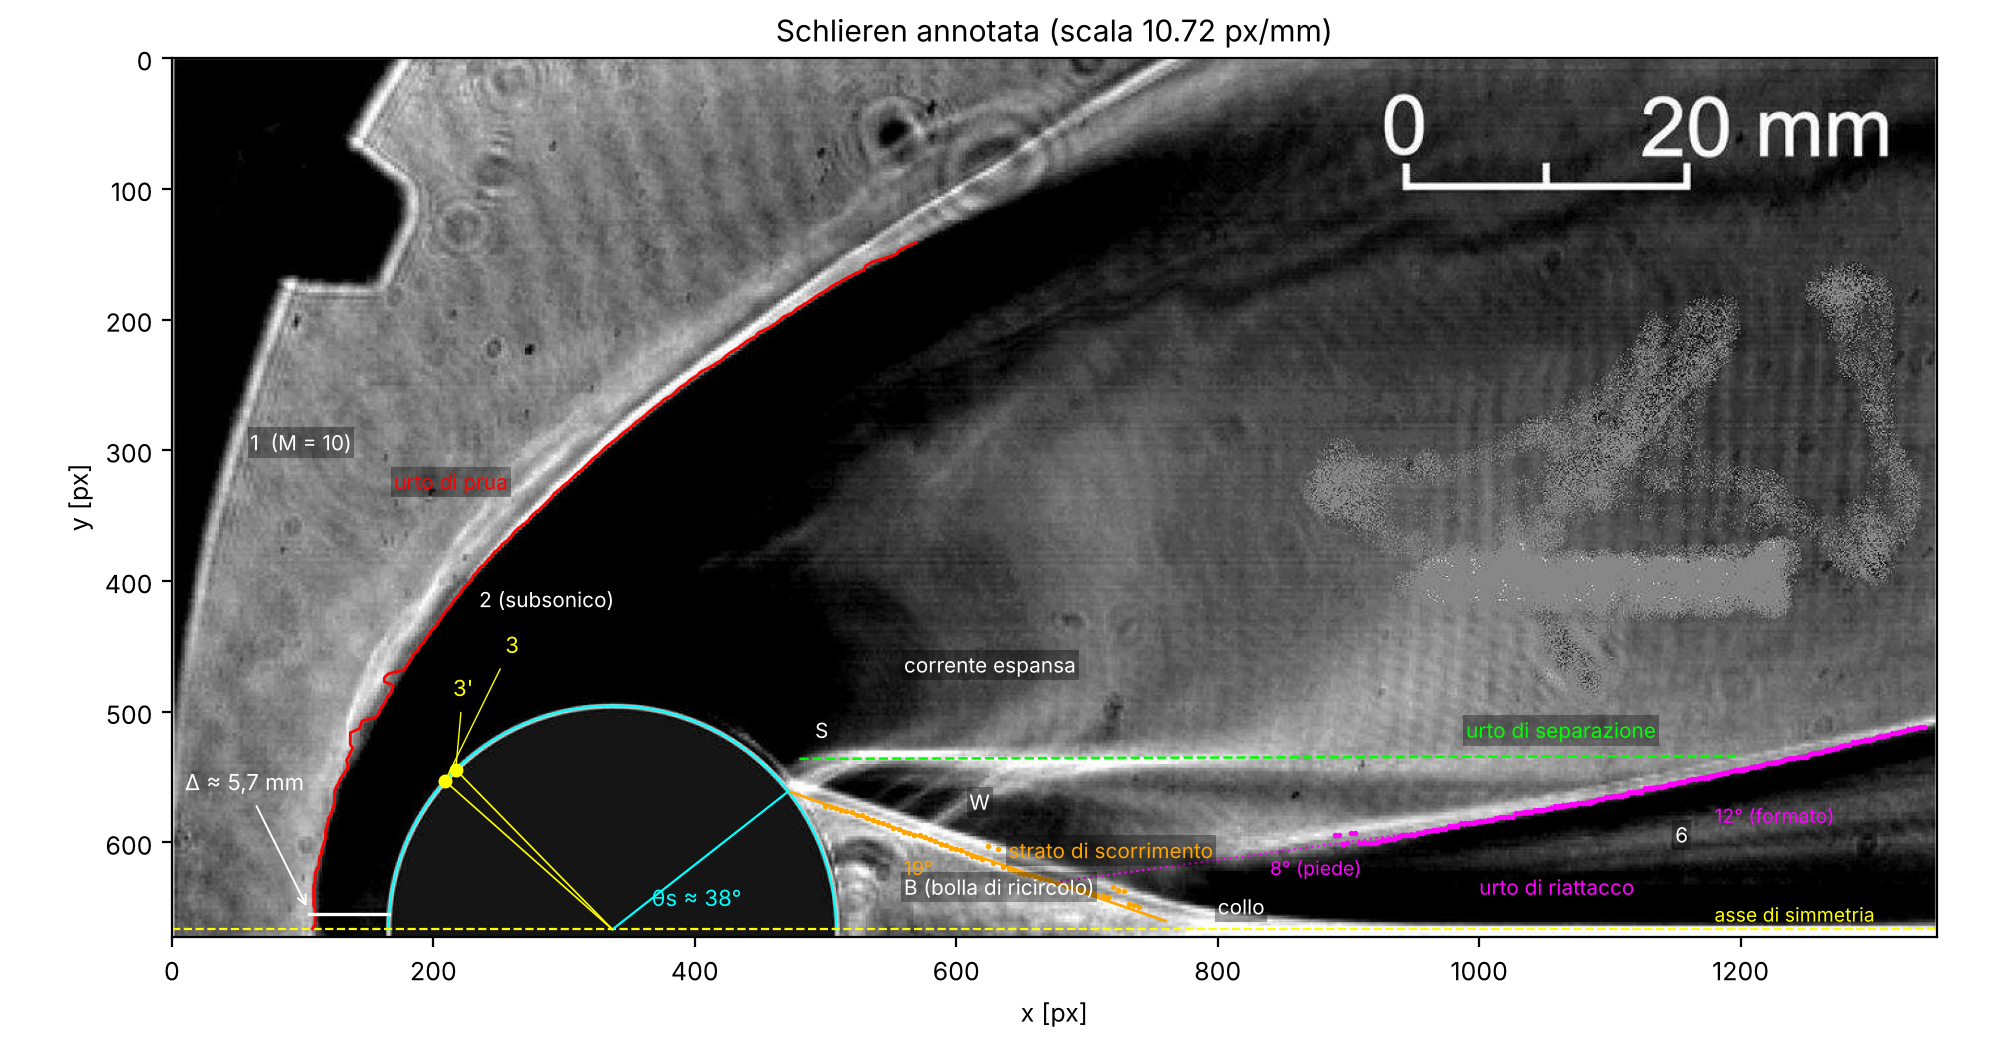
\includegraphics[width=\textwidth]{annotata.png}
  \caption{Schlieren annotata. In rosso l'urto di prua tracciato; in arancio i punti dello strato di
  scorrimento e la retta del primo tratto (\ang{19}); in magenta i punti dell'urto di riattacco, con
  il tratto formato (\ang{12}) e il piede (\ang{8}, punteggiato); in verde l'urto di separazione (circa \ang{0}).
  Sono indicati la stand-off, l'angolo di separazione $\theta_s$, i punti sonici 3 (catena) e 3$'$
  (Busemann) e gli stati 1, 2, S, W, B, 6.}
  \label{fig:ann}
\end{figure}
\textbf{Commento (fig.~\ref{fig:ann}).} Tutte le strutture della §2 sono state ritrovate e misurate. Lo strato di
scorrimento tracciato si sovrappone bene alla banda chiara del contorno della bolla. Le rette adattate seguono
le linee entro 1--3 px di scarto tipo. I due punti sonici stimati sono vicini fra loro (circa \SI{1}{mm} sul
contorno) e stanno nella parte del cilindro dove l'urto di prua comincia a inclinarsi in modo
marcato.

\begin{figure}[H]
  \centering
  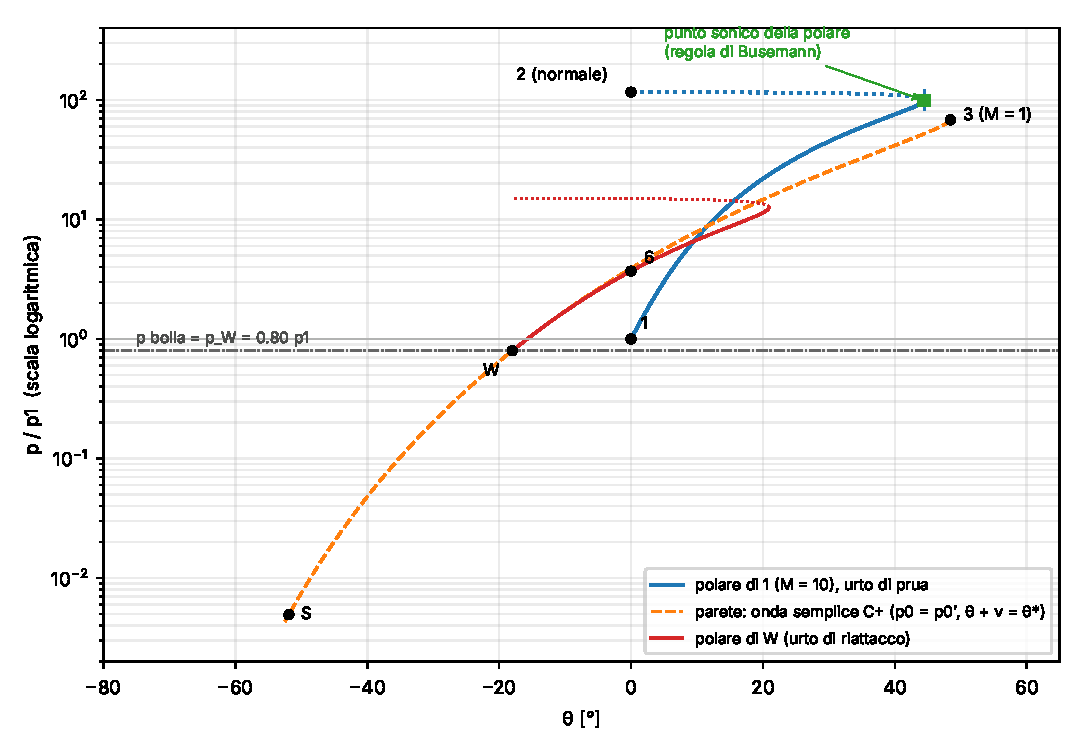
\includegraphics[width=0.85\textwidth]{p_theta.pdf}
  \caption{Piano $p$--$\theta$ (pressione in scala logaritmica). Polare di 1 (urto di prua, $\Cp$, metà
  superiore); curva isentropica della corrente di parete ($p_0=p_0'$, $\theta+\nu=\theta^*$); polare di W (urto di
  riattacco); pressione della bolla.}
  \label{fig:pth}
\end{figure}
\textbf{Commento (fig.~\ref{fig:pth}).} La polare di 1 \emph{non parte dall'origine}: parte da $(0,\,1)$
(onda nulla) e sale fino allo stato 2 (urto normale, $p=116{,}5\,p_1$, ramo forte punteggiato). Lungo
l'urto di prua il campo a valle percorre tutta la polare, dal ramo forte vicino all'asse al ramo debole lontano dal corpo.
Il quadratino è il punto sonico della polare, che usa la regola di Busemann. Lo stato 3 ($M=1$ a parete) sta
\emph{sotto} quel punto: la linea di parete ha la $p_0'$ dell'urto normale, più bassa della pressione totale a valle di un urto obliquo.
Questo mostra che la linea sonica non è un'isobara. Dalla curva tratteggiata di parete si scende con l'espansione
fino a S ($\theta=-\ang{52}$, $p=\num{4.9e-3}$). La compressione isentropica riporta lungo la \emph{stessa}
curva fino a W ($\theta=-\ang{18}$, $p=0{,}80$), che fissa la pressione della bolla (retta tratteggio-punto).
Da W parte la polare dell'urto di riattacco, che taglia $\theta=0$ nello stato 6 sul ramo debole. La scala
logaritmica, necessaria per l'escursione di cinque ordini di grandezza, deforma la concavità dei rami.

\begin{figure}[H]
  \centering
  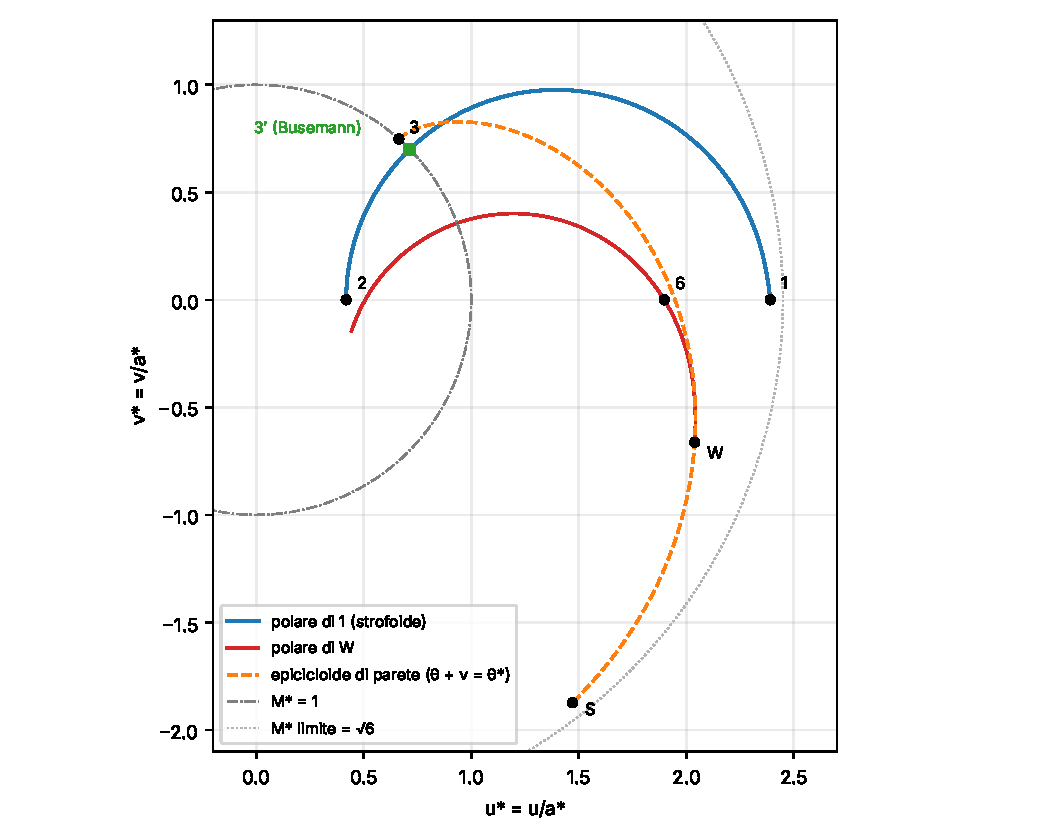
\includegraphics[width=0.75\textwidth]{odografo.pdf}
  \caption{Piano odografo $(u^*,v^*)=(V/a^*)(\cos\theta,\sin\theta)$, con $a^*$ unico ($h_0$ uniforme):
  strofoide di 1, epicicloide di parete per $\theta+\nu=\theta^*$, polare di W, cerchio sonico e cerchio limite.}
  \label{fig:od}
\end{figure}
\textbf{Commento (fig.~\ref{fig:od}).} Lo stato 1 è sull'asse $u^*$ a $M^*_1=2{,}39$, poco dentro il
cerchio limite $\sqrt6$ (a $M=10$ la velocità è già vicina alla velocità limite). La strofoide va da 1
allo stato 2 ($M^*_2=0{,}418$, dentro il cerchio sonico) e taglia il cerchio sonico nel punto 3$'$ di
Busemann. Il punto sonico 3 a parete sta sul cerchio sonico a $\theta^*=\ang{48.4}$. Da 3 parte
l'epicicloide di Prandtl--Meyer: la percorro verso destra-in basso fino a S ($M^*=2{,}38$, vicino al
cerchio limite: espansione quasi totale), poi indietro fino a W ($M^*=2{,}14$). Infine la polare di W porta allo stato 6
sull'asse ($M^*=1{,}90$).

%==============================================================================
\section{Discussione fisica}\label{sec:disc}
\paragraph{Struttura del campo.} È quella tipica di un corpo tozzo ipersonico. Davanti c'è un urto staccato,
normale sull'asse, con una bolla subsonica al naso (non si parla di ``transonico'': la corrente lontana è supersonica).
Lungo il corpo c'è un'espansione molto forte. Dietro ci sono la separazione con l'urto di separazione, la bolla di ricircolo
a bassa pressione, il collo e l'urto di riattacco. Tutto ciò che sta a valle della linea sonica non può
influenzare il naso: la stand-off e la forma dell'urto anteriore dipendono solo dalla regione subsonica.
Per questo una scia instazionaria non disturba la parte anteriore dell'immagine.

\paragraph{Perché il tratto ``formato'' dell'urto di riattacco.} Con l'inclinazione del piede
($\sigma_{ax}=\ang{7.8}$, $\sigma=\ang{25.8}$) si otterrebbe $M_W=6{,}1$, $\theta^*=\ang{67.7}$ e un punto sonico a
$\theta_c=\ang{22}$, oltre \ang{20} lontano dalla regola di Busemann. Quindi il piede non è utilizzabile.
Un'inclinazione al piede di circa \ang{10} (quella che si ottiene a occhio prendendo il primo
tratto) darebbe $M_W\simeq4{,}8$ e $\theta_c\simeq\ang{32}$, comunque fuori dall'accordo. La lettura coerente è che l'urto
porta tutta la deviazione solo dopo la coalescenza. È la stessa fisica della compressione su parete concava, e
spiega anche la curvatura visibile dell'urto.

\paragraph{Limiti del modello di parete.} La catena dà $p_S\approx5\cdot10^{-3}\,p_1$ e $M_S\approx9$: valori
estremi, perché l'onda semplice lungo la parete trascura le onde riflesse dall'urto di prua, dalla linea sonica
e dallo strato d'entropia, oltre allo strato limite che si ispessisce. Nella realtà l'espansione a parete è meno
spinta. Per questo c) è il risultato più incerto: $d\nu/dM\to0$ per $M\to\infty$, e l'intervallo
7--13,5 riflette proprio questa sensibilità. Il punto sonico, invece, si ricava senza passare da S
(invariante $\theta+\nu$ fra 3 e W) ed è molto più robusto.

\paragraph{Entropia e vorticità.} Le linee di corrente vicine al corpo, che hanno attraversato l'urto quasi
normale, hanno $p_0'=129\,p_1$. Quelle più esterne hanno pressioni totali molto più alte (fino a $p_{01}=4{,}2\cdot10^4\,p_1$
lontano). Il campo dietro l'urto curvo è rotazionale (Crocco). Il modello usato (corrente W uniforme con
$p_0'$) vale per lo strato adiacente alla scia, non per tutta la corrente esterna. In particolare non vale sopra
l'urto di separazione, ed è per questo che oltre l'incrocio l'urto di riattacco cambia inclinazione.

\paragraph{Viscosità.} La posizione della separazione, e quindi $\theta_R$, $M_S$, l'estensione della bolla e $p_B$,
dipende dallo strato limite (numero di Reynolds): una teoria non viscosa non la prevede, la misura sì.
La pressione di base trovata ($0{,}5$--$1{,}2\,p_\infty$) è dell'ordine atteso per una base ipersonica. Dato che
la resistenza è dominata dalla pressione al naso ($p_0'=129\,p_1$), l'errore su $p_B$ pesa poco sulla resistenza.

\paragraph{Gas reale.} A $M=10$ in galleria la temperatura statica è molto bassa e la temperatura di
ristagno moderata: l'ipotesi di gas perfetto con $\gamma=1{,}4$ è ragionevole. In volo, alla stessa $M$,
dietro l'urto normale ci sarebbero dissociazione e $\gamma$ efficace minore. Ne seguirebbero un urto più vicino al corpo
(rapporto di densità maggiore) e una stand-off più piccola.

\end{document}
